\section{Machine Learning e Deep Learning}
Il \textbf{\textit{machine learning}} è una branca dell'intelligenza artificiale (AI) che si occupa in generale di fornire ad una macchina la capacità di apprendere automaticamente dall'esperienza, essendo esplicitamente programmata su "come imparare" ma non su "cosa imparare".

Questa capacità è fornita da un certo algoritmo di machine learning, di cui T. Mitchell fornisce una celebre ed elegante definizione:
\begin{quote}
Si dice che un programma per computer impara dall’esperienza E rispetto ad una qualche classe di compiti T ed una misura di performance P se le sue prestazioni nei compiti in T, misurate attraverso P, migliorano con l’esperienza E.
\end{quote}

L'obiettivo principale dell'apprendimento automatico è che una macchina sia in grado di generalizzare dalla propria esperienza\cite{bishop}, ossia che sia in grado di svolgere ragionamenti induttivi. In questo contesto, per generalizzazione si intende l'abilità di una macchina di portare a termine in maniera accurata esempi o compiti nuovi, che non ha mai affrontato, dopo aver fatto esperienza su un insieme di dati di apprendimento.
Gli esempi di addestramento (in inglese chiamati \textit{training examples}) si assume provengano da una qualche distribuzione di probabilità, generalmente sconosciuta e considerata rappresentativa dello spazio delle occorrenze del fenomeno da apprendere; la macchina ha il compito di costruire un modello probabilistico generale dello spazio delle occorrenze, in maniera tale da essere in grado di produrre previsioni sufficientemente accurate quando sottoposta a nuovi casi.

Quasi tutti gli algoritmi di machine learning sono costruiti combinando almeno quattro
building blocks fondamentali: un dataset, un modello, una funzione costo ed un
metodo di ottimizzazione.\\

Il \textbf{\textit{deep learning}} è un tipo specifico di machine learning, che negli ultimi anni ha dato una svolta decisiva alla più vasta branca dell’intelligenza artificiale.

Un algoritmo di deep learning si basa su diversi livelli di rappresentazione dei dati, che corrispondono a differenti livelli di astrazione; questi livelli formano una gerarchia di concetti, in cui i concetti di più alto livello sono definiti sulla base di quelli di livello più basso.

Il modello computazionale utilizzato in maniera esclusiva nel \textit{deep learning} è la rete neurale artificiale (par. \ref{ANN})\\

Il deep learning è inquadrato in una più ampia branca del machine learning, chiamata \textbf{\textit{representation learning}}. Nell'ambito del representation learning, l'approccio usato per la risoluzione dei problemi consiste non solo nel tentare di addestrare un computer a trovare una relazione tra dati e output, ma anche nel fornirgli strumenti per la rappresentazione stessa dei dati, in quanto in alcuni contesti il legame tra i dati in input e quelli attesi in output è tutt'altro che lineare ed è in generale complesso, e può essere più facile per la macchina acquisire diversi livelli di conoscenza e di astrazione dei dati in input per calcolare l'output.

Si pensi ad esempio ad un task di \textit{image classification}. È impensabile descivere la presenza di un oggetto all’interno di un'immagine attraverso un legame lineare con i singoli pixel. È piuttosto la combinazione di pixel l'informazione da mappare (in maniera in generale non lineare) con la categoria di appartenenza di quell'oggetto.

Dagli studi scientifici sull'apparato visivo sappiamo che l'uomo riesce a riconoscere gli oggetti attraverso una rappresentazione gerarchica degli stessi:

\begin{itemize}
\item dapprima captiamo caratteristiche di basso livello degli oggetti che vediamo, come forme (spigoli, angoli) e tonalità di colore. Tutte queste caratteristiche sono "locali", nel senso che occupano una regione limitata del campo visivo, essendo parti più piccole dell'oggetto. In questa fase, non sappiamo ancora dare un nome all'oggetto su cui ci concentriamo;
\item queste caratteristiche (\textit{features}) sono combinate nella parte del cervello che si occupa della visione, a formare concetti di più alto livello come il perimetro dell'oggetto e le sfumature (gradienti) di colore;
\item questa rappresentazione graduale e gerarchica dei concetti, arrivata a concetti di più alto livello, permette infine di associare alla "immagine" formatasi nel nostro campo visivo il nome dell'oggetto, o degli oggetti, in esso presenti.
\end{itemize}

Sulle medesime basi "biologiche" si fondano le reti neurali artificiali, attraverso gli \textit{hidden layers} (strati nascosti) frapposti tra l'input e l'output della rete stessa che permettono di combinare le informazioni provenienti dagli strati precedenti per ottenere una rappresentazione dei dati di più alto livello.

\begin{figure}[h]
\centering
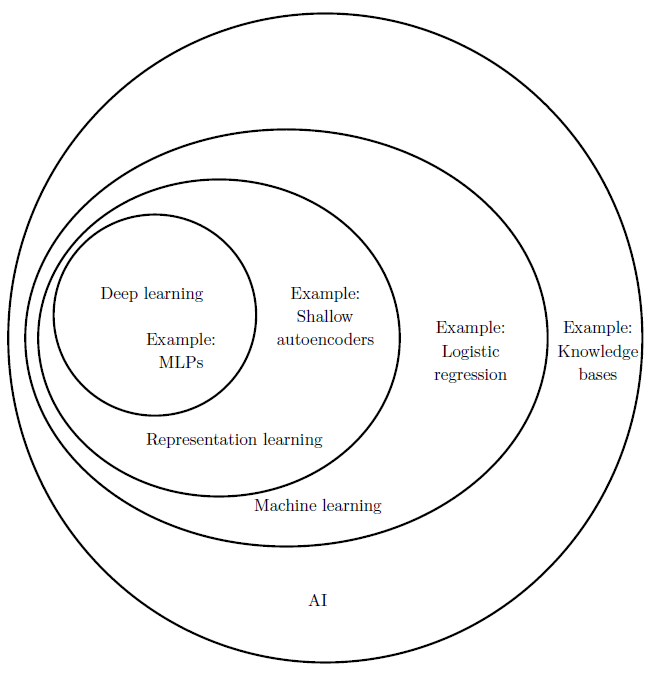
\includegraphics[width=0.7\textwidth]{diagrammaIA}
\caption{Un diagramma di Venn che mostra come il deep learning sia un tipo di
representation learning, che a sua volta è un tipo di machine learning.}
\label{diagrammaAI}
\end{figure}


\subsection{Supervised Learning}
\label{supervisedLearning}

Il paradigma dell'\textbf{apprendimento supervisionato} (\textit{supervised learning}) mira alla creazione di un algoritmo che analizzi dei "dati di addestramento", una collezione di esempi ideali costituiti da coppie di input e relativi output attesi, e da questi inferisca una funzione che può essere usata per mappare nuovi input ai corretti output \cite{Russell2009}.
Ciò richiede all'algoritmo la capacità di trovare una funzione che sappia generalizzare efficacemente dai dati di training, al fine di adattarsi bene a nuovi dati (per poterne mappare correttamente quanti più possibile).\\

Molti problemi pratici, come ad esempio la regressione e la classificazione delle immagini (par. \ref{objectRecognition}, possono essere formulati ricorrendo ad una funzione matematica
\[\mathcal{F}:X\to Y\]
che associa ad ogni elemento dello spazio degli input $X$ uno ed un solo elemento dello spazio degli output $Y$.
Il concetto di funzione implica l'esistenza di un solo elemento di $Y$ a cui ogni elemento di $X$ è correttamente associato. Il problema consiste allora nel cercare una funzione $\mathcal{F}$ in grado di ottenere esattamente tale associazione, per quanti più elementi di $X$ possibile.

È evidente che questo tipo di problemi ben si presta ad essere approcciato con algoritmi di apprendimento supervisionato.

Prima di analizzare in dettaglio il problema di classificazione delle immagini oggetto della presente tesi, è necessario inquadrare il problema partendo da alcune definizioni preliminari.\\

Un \textbf{dataset} X è una generica collezione di $N$ dati
\[X=\{\mathbf{x}^{(1)},\mathbf{x}^{(2)},\dots,\mathbf{x}^{(N)}\}\]
Ogni dato $\mathbf{x}^{(i)}$ è chiamato \textbf{esempio} (o \textbf{data point}).
I data point possono essere anche non omogenei tra loro (cioè avere dimensioni differenti).
Ciascun esempio si può caratterizzare come un vettore $\mathbf{x}^{(i)}\in\R^{D}$, in cui ciascun elemento $x_i$ è detto \textbf{feature} e rappresenta una caratteristica di un oggetto o un evento misurato. $D$ è il numero di feature in ogni esempio, o \textbf{dimensione} dell'esempio.
In caso di esempi omogenei (cioè aventi stessa dimensione $D$) un dataset può essere descritto attraverso una matrice detta \textbf{design matrix}, in cui ogni riga corrisponde ad un particolare esempio e ogni colonna corrisponde ad una precisa feature.
Un dataset di cardinalità $N$ e in cui ogni esempio ha $D$ feature ha quindi una design matrix di dimensione $N\times D$. \\

In un problema di classificazione delle immagini sussiste la seguente caratterizzazione:
\begin{itemize}
\item $X$: un insieme di $N$ immagini digitali
\item $Y$: un insieme di $K$ classi predefinite di oggetti che possono essere individuati all'interno di un'immagine (possono essere dei "descrittori" testuali o, equivalentemente, dei numeri interi)
\end{itemize}
Un elemento di $Y$ è solitamente chiamato \textbf{etichetta} o \textbf{categoria} (in inglese \textbf{label} o \textbf{class}); si dice quindi che ogni immagine $\mathbf{x}^{(i)}\in X$ può essere \textit{descritta da un'etichetta} (o \textit{associata ad una categoria}) $\mathbf{y}^{(i)}\in Y$ tramite una funzione di associazione $f$.\footnote{Teoricamente una stessa immagine potrebbe essere descritta da più di un'etichetta o addirittura da nessuna, coerentemente col fatto che in essa potrebbero essere presenti più oggetti o nessun oggetto tra quelli previsti in $Y$. Tuttavia nella presente tesi questa ambiguità non può sussistere: la classificazione riduce qualsiasi immagine ad una di due categorie mutualmente esclusive e di cui soltanto una è quella corretta, cioè la presenza o meno di una pinna nell'immagine.}\\

Tipicamente, per l'addestramento di un modello di machine learning si usa un sottoinsieme del dataset $X$ a disposizione. Questo sottoinsieme $X^{train}$ è definito \textbf{\textit{training set}}.

Nella pratica, l'espressione analitica di $f$ non può essere trovata esattamente. Ad esempio, nel problema in esame, non è chiaro come poter scrivere un algoritmo che consenta di individuare con esattezza la presenza di una pinna all'interno di un'immagine, poiché il concetto di "pinna" non è un concetto matematico e non può essere reso facilmente in un linguaggio "comprensibile" da un computer. Inoltre, il computer può disporre solamente di un numero limitato $\left|X^{(train)}\right|$ di esempi, cioè un numero limitato di occorrenze di oggetti di tipo "pinna", che non permettono di generalizzare a tutte le forme ed i colori in cui una pinna può essere presente in un'immagine. Per questo motivo, ciò che il modello di machine learning da addestrare è chiamato ad imparare è un'approssimazione quanto più "plausibile" di $f$, dove per "plausibilità" si intende la capacità della funzione trovata di restituire il giusto output per il maggior numero possibile di input presentati.

\subsection{Underfitting e overfitting}
\label{overfitting}
La sfida principale dell'apprendimento automatico è quella di rendere l'algoritmo di machine learning performante su nuovi input, diversi da quelli su cui il modello è stato addestrato. Questa abilità è chiamata \textbf{generalizzazione}.\\

Tipicamente, dopo l'addestramento di un modello di machine learning con un \textit{training set} possiamo misurare le performance del modello con un parametro detto \textit{training error}, definito come il rapporto tra il numero di esempi del training set che alla fine dell'addestramento l'algoritmo associa al giusto output, $\left|X_{corrette}\right|<\left|X\right|$, e la dimensione del \textit{training set}, $\left|X\right|$:
\[\text{Training Error}=\frac{\left|X_{corrette}\right|}{\left|X\right|}\]
Ovviamente, con l'addestramento si vuole minimizzare questo rapporto. Quello descritto è un problema di ottimizzazione.\\

Tuttavia non basta che il modello si comporti bene su una collezione di dati di cui fondamentalmente si conosceva già l'output (abilità di per sé abbastanza inutile), ma si vuole, come già spiegato, che esso lavori bene anche su un \textbf{test set} $T$ di esempi mai forniti in input per l'addestramento del modello, e pertanto non presenti nel training set. Si può definire similmente al \textit{training error} un parametro detto \textbf{\textit{generalization error}} (errore di generalizzazione), o \textbf{\textit{test error}}.
\[\text{Test Error}=\frac{|T_{corrette}|}{|T|}\]
Si vuole ovviamente che anche il test error, come il training error, sia piccolo. Più precisamente, si vuole che la differenza tra il training error e il test error sia quanto più piccola possibile.\footnote{Il problema di ottimizzazione da risolvere è quello della minimizzazione del training error. Il test error non può essere minimizzato, in quanto esso viene valutato quando l'addestramento della rete è finito; anche in fase di training, comunque, il test set non è disponibile per l'addestramento (non può essere trattato come un'estensione del training set, pena la violazione della definizione stessa di "test set").}\\

I fattori che determinano quanto bene un algoritmo di machine learning performerà sono in definitiva le sue capacità di
\begin{enumerate}
\item rendere piccolo il training error
\item rendere piccola la differenza tra training error e test error
\end{enumerate}

Quando un modello non riesce ad ottenere un errore sufficientemente basso sul training set si dice che il modello soffre di \textbf{\textit{underfitting}} (sottoadattamento). Quando il modello non riesce a rendere piccola a sufficienza la differenza tra training error e test error si dice che il modello soffre di \textbf{\textit{overfitting}} (sovradattamento).

Possiamo controllare la tendenza di un modello all'underfitting o all'overfitting  regolando la sua \textbf{capacità}. Informalmente, la capacità di un modello è la sua abilità ad adattarsi ad un insieme ampio di funzioni. Modelli con capacità bassa potrebbero avere difficoltà nell'adattarsi al training set (underfitting). Al contrario, modelli con capacità alta hanno una maggiore probabilità di adattarsi troppo bene al training set (overfitting), memorizzando molte caratteristiche e proprietà degli esempi del training set che non sempre aiutano nella generalizzazione ai nuovi casi, ad esempio quelli del test set.

In una rete neurale (par. \ref{ANN}) la capacità del modello può essere definita, ad esempio, come il numero di parametri addestrabili (pesi e bias) che la caratterizzano.

Gli algoritmi di machine learning performeranno generalmente bene quando la loro capacità è appropriata rispetto alla reale complessità del task che devono svolgere e alla quantità di esempi $|X^{train}|$ forniti per l'addestramento. Modelli con una capacità insufficiente non riescono a risolvere task complessi. Modelli con alta capacità possono risolvere task complessi, ma se la loro capacità è eccessivamente alta rispetto alla complessità del task in esame potrebbero soffire di overfitting. La fig. \ref{fig:capacity} presenta bene la situazione.

\begin{figure}[h]
\centering
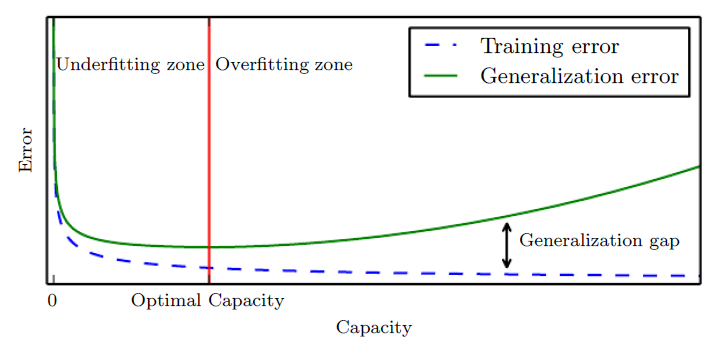
\includegraphics[width=0.8\textwidth]{capacity}
\caption{Training error e test error (asse y) al variare della capacità del modello (asse x)}
\label{fig:capacity}
\end{figure}

Negli esperimenti condotti una delle reti neurali utilizzate (ResNet-50) ha sofferto di overfitting a causa della sua enorme capacità di rappresentazione e del training set relativamente ristretto usato per il suo addestramento (par. \ref{addestramento}).

\section{Classificazione}
\label{classificazione}
In un problema di classificazione l’insieme delle classi $Y$ è discreto e finito.
Sulla base del numero di classi $|Y|$ si distinguono due tipi di classificazione: binaria ($|Y|=2$) o multiclasse ($|Y|>2$).

TODO magari lo inserisco direttamente nel capitolo sulle reti neurali.








\section{Classificatore lineare}
\label{classificatoreLineare}
Il classificatore lineare è uno tra i più semplici modelli di classificazione.
Ipotizziamo di avere un insieme di $N$ immagini $\mathbf{x}^{(i)}$ (\textit{data points}), ciascuna con risoluzione fissa $w\times h$ e in formato RGB ($c=3$), e un insieme di $K$ distinte categorie di oggetti  (\textit{labels}). Un \textbf{classificatore lineare} è definito dalla funzione
\begin{equation} \label{eq_class_lin}
f(\mathbf{x}^{(i)};\mathbf{W},\mathbf{b})=\mathbf{W}\mathbf{x}^{(i)}+\mathbf{b}
\end{equation}
In questa espressione stiamo assumendo che $\mathbf{x}^{(i)}$ sia un vettore colonna di dimensione $D=hwc$ ottenuto incolonnando una ad una le righe dell'$i$-esima immagine di tutti e tre i canali di colore, $\mathbf{W}$ una matrice detta \textbf{matrice dei pesi} (\textit{weights matrix}) di dimensione $K\times D$ e $\mathbf{b}$ un vettore colonna detto \textbf{vettore dei bias} (\textit{bias vector}) di dimensione $K$. I pesi e i bias sono parametri della funzione $f$.

Ogni riga $j$-esima di $W$ e il relativo $j$-esimo valore di $\mathbf{b}$ serve a calcolare la combinazione (lineare a meno del bias) $\mathbf{w}_j\cdot \mathbf{x}^{(i)}+b_j$. Ognuna delle $K$ combinazioni calcolate è un numero reale che si può interpretare come un "punteggio" registrato dall'$i$-esima immagine in ogni classe di oggetti in $Y$ (\textit{class score}): l'$i$-esima immagine è classificata con l'etichetta $\mathbf{y}_j\in Y$ se l'elemento $j$-esimo del vettore output $f(\mathbf{x}^{(i)};\mathbf{W},\mathbf{b})$ è il massimo del medesimo vettore.\\

L'esempio in figura \ref{class_lin} mostra la classificazione di un'immagine di un gatto con $\abs{Y}=3$ classi (\textit{gatto}, \textit{cane}, \textit{barca}). Per semplicità, l'immagine input è ipotizzata $2\times 2$ e composta da un unico canale di colore ($c=1$) (quindi $\mathbf{x}$, scritta come vettore colonna, è $4\times 1$).

\begin{figure}[h!]
\centering
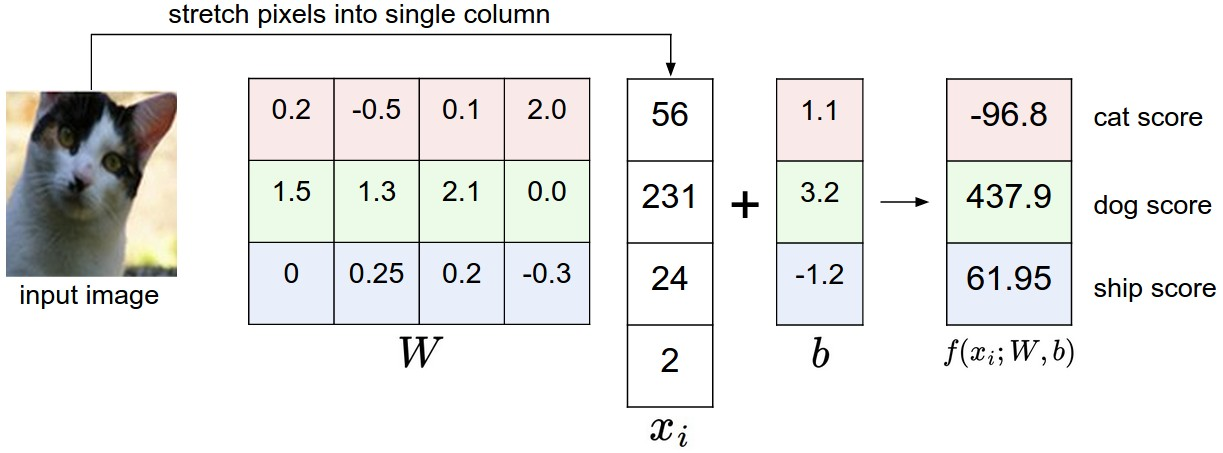
\includegraphics[width=\textwidth ,keepaspectratio]{classificatore_lineare}
\caption{Mappatura di un'immagine ai punteggi di ogni classe mediante un classificatore lineare. Si noti che i pesi di $\mathbf{W}$ non costituiscono un buon set di parametri: il punteggio assegnato alla classe "cane" (sbagliata) è alto e quello totalizzato dalla classe "gatto" (corretta) è basso. Il classificatore "è convinto" di aver classificato l'immagine di un cane.}
\label{class_lin}
\end{figure}

Come si vedrà nel par. \ref{neuroni}, nelle reti neurali il classificatore lineare sarà utilizzato come un singolo "blocco da costruzione" per costruire una rete più grande.

\subsection*{Interpretare un classificatore lineare}

Poiché le immagini possono essere memorizzate come vettori colonna $hwc$-dimensionali, si possono immaginare le immagini di un dataset come dei punti nello spazio $\R^{hwc}$. Di conseguenza, il dataset può essere pensato come una collezione di punti multidimensionali. Ovviamente non possiamo visualizzare spazi con più dimensioni di $\R^{3}$, ma se immaginiamo di "comprimere" tutte le $hwc$ dimensioni in sole due dimensioni otteniamo una visualizzazione del tipo in figura \ref{visual_class_lin}.

\begin{figure}[h]
\centering
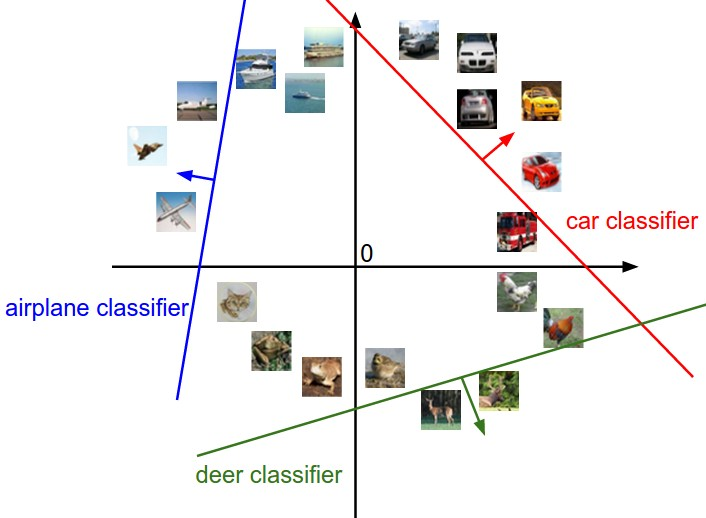
\includegraphics[width=\textwidth ,keepaspectratio]{visualizz_class_lin}
\caption{Visualizzazione di tre righe di un classificatore lineare, una per ciascuna delle classi "aereo", "auto", "cervo".}
\label{visual_class_lin}
\end{figure}

Le rette in figura devono in realtà essere pensate come degli iperpiani $(hwc-1)$-dimensionali, associati a ciascuna classe di $Y$ (cioè a ciascuna riga di $\mathbf{W}$ e $\mathbf{b}$), e il piano come lo spazio $\R^{hwc}$. Sussistono le seguenti interpretazioni geometriche:
\begin{itemize}
\item Le immagini sono dei punti nel piano. Ogni retta è il luogo dei punti che totalizzano un punteggio nullo per la classe associata a quella retta (la classe è scritta in figura accanto ad ogni retta). La freccia nella figura indica la direzione seguendo la quale i punti del piano aumentano (linearmente) il punteggio realizzato per quella classe.
\item Modificare i pesi di $\mathbf{W}$ significa regolare l'inclinazione delle rette (cioè ruotarle rispetto al punto di intercetta).
\item Modificare i bias di $\mathbf{b}$ significa regolare l'intercetta delle rette (cioè traslarle verticalmente).
\end{itemize}

Un altro modo di interpretare i pesi $\mathbf{W}$ può essere quello di far corrispondere ogni riga di $\mathbf{W}$ a un \textbf{prototipo} (in inglese \textbf{template}) per una delle classi. In questa interpretazione, il punteggio realizzato per ogni classe da un'immagine è ottenuto attraverso l'operazione di prodotto matriciale tra il prototipo della classe $j$ ($\mathbf{w}_j$) e l'immagine da classificare ($\mathbf{x}^{(i)}$).
Usando la terminologia introdotta, possiamo affermare che ciò che sta facendo il classificatore lineare è un'operazione di \textit{template matching}, dove i \textit{templates} sono oggetto di apprendimento da parte del classificatore\footnote{Si introdurranno gli algoritmi di apprendimento (supervisionato) nel paragrafo \ref{supervisedLearning}.}.

Ad esempio, analizziamo il dataset \textit{CIFAR-10} \cite{cifar10}. Esso contiene immagini $32\times 32$ ciascuna appartenente ad una di 10 classi. Visualizzando\footnote{TODO Per i dettagli su come "visualizzare" i pesi si veda \url{https://it.mathworks.com/help/deeplearning/examples/visualize-activations-of-a-convolutional-neural-network.html}.} i pesi (e quindi i 10 templates) di un classificatore lineare addestrato su CIFAR-10 si ottengono i risultati in figura seguente:

\begin{figure}[h]
\centering
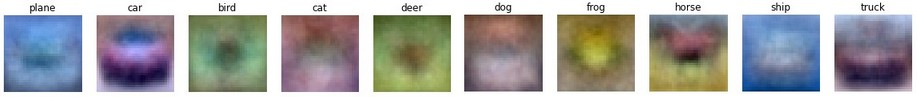
\includegraphics[width=\textwidth ,keepaspectratio]{templates}
\caption{Visualizzazione dei templates di un classificatore addestrato sul dataset CIFAR-10}
\label{templates}
\end{figure}

Si possono fare alcune interessanti osservazioni.

Ad esempio, il prototipo della classe "barca" è composto da molti pixel blu disposti perlopiù lungo i margini, come ci si potrebbe aspettare dal momento che molte immagini di barche in CIFAR-10 raffigurano queste in mare aperto. Questo template allora assegnerà un punteggio alto quando l'immagine che si vuole classificare (cioè \textit{raffrontare al template}) è una barca in mare aperto. In altre parole, un'immagine realizzerà un punteggio tanto più alto in una certa classe quanto più essa è \textit{simile} al template che il classificatore lineare \textit{ha imparato} per quella classe.

Il prototipo per la classe "cavallo" sembra essere l'immagine di un cavallo a due teste; similmente, quello per la classe "auto" sembra una miscela di rappresentazioni di un'auto vista da più direzioni diverse. Ciò è coerente col fatto che il classificatore lineare è stato addestrato su immagini di cavalli visti rispetto a entrambi i profili e su immagini
di auto raffigurate in tante direzioni diverse. Inoltre, il template per l'auto sembra rappresentare un'auto di colore rosso: evidentemente in CIFAR-10 la maggior parte delle automobili rappresentate sono di quel colore.\\

Come si vedrà nel seguito, questa operazione di \textit{template matching} presenta una forte analogia con il funzionamento di un \textit{Fully Connected Layer} di una rete neurale convoluzionale.

\subsection*{Bias trick}
Concludiamo questo capitolo menzionando un "trucco" matematico molto utilizzato per rappresentare $\mathbf{W}$ e $\mathbf{b}$ come un'unica matrice, semplificando la notazione \ref{eq_class_lin}.
Possiamo aggiungere il vettore dei bias in coda alla matrice dei pesi e aggiungere un "1" in coda al vettore che rappresenta l'immagine. In questo modo, il classificatore lineare è rappresentato dalla funzione di associazione
\begin{equation} \label{eq_bias_trick}
f(\mathbf{x}^{(i)};\mathbf{W})=\mathbf{W}\mathbf{x}^{(i)}
\end{equation}

In questa maniera, $f$ calcola solo combinazioni lineari (un singolo prodotto matriciale), poiché il vettore dei bias è stato eliminato.
Tale utile passaggio, noto come \textit{bias trick}, è visualizzato nella seguente figura

\begin{figure}[h]
\centering
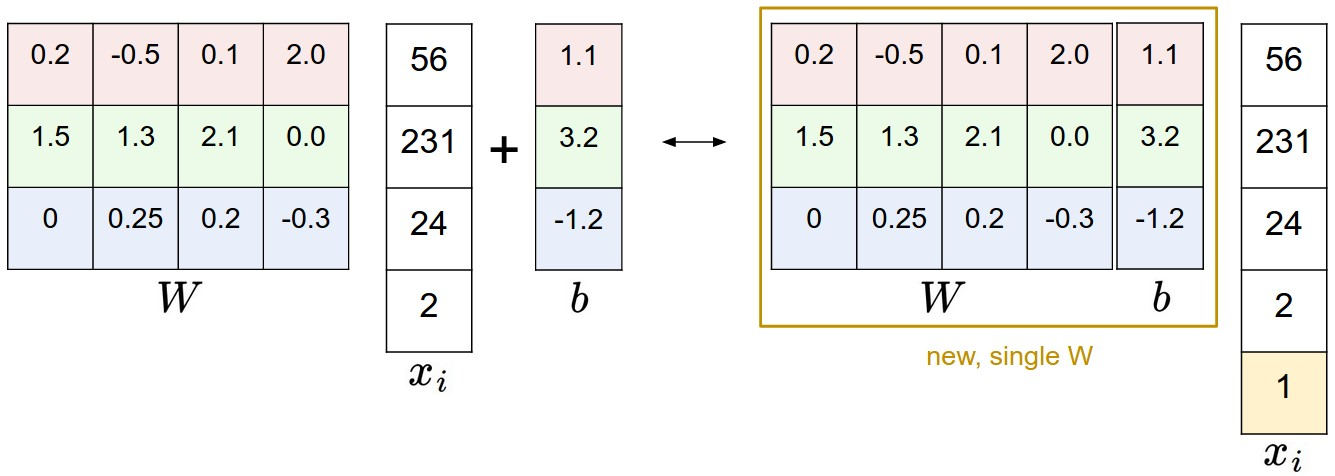
\includegraphics[width=\textwidth ,keepaspectratio]{bias_trick}
\caption{Bias trick}
\label{bias_trick}
\end{figure}

TODO: loss functions.

TODO: valutazione delle prestazioni di una rete neurale (matrice di confusione)


